\documentclass{article}
\usepackage[a4paper, total={180mm, 260mm}]{geometry}
\usepackage{graphicx}
\usepackage{url}
\usepackage{natbib}
\usepackage{todonotes}
\usepackage{booktabs}
\usepackage{lineno}
\usepackage{color}
%\usepackage{auto-pst-pdf}
\usepackage[colaction]{multicol}
\usepackage{caption}
\usepackage{svg}
\usepackage{authblk}
\usepackage{standalone}

\usepackage[section]{placeins}


\linespread{1.5}

\makeatletter
\renewcommand{\maketitle}{\bgroup\setlength{\parindent}{0pt}
	\begin{flushleft}

		{\huge\textbf{\@title}}

		\bigskip

 		{\large\textbf{\@author}}

 		\bigskip

 		{\large{Draft current \@date}}

	\end{flushleft}\egroup
}
\makeatother

\newcommand{\multicollinenumbers}{
	\linenumbers
	\def\makeLineNumber{\docolaction
		{\makeLineNumberLeft}
		{}
		{\makeLineNumberRight}
		}
}

\newenvironment{figurehere}
	{\def\@captype{figure}}
	{}

% Title
\title{A Topic Model of Climate Change Literature}
\title{Words, words, words: Mapping the Matter of Climate Change Literature}
\title{A Topography of Climate Change Research}
\author[1,2]{Max Callaghan}

\affil[1]{Mercator Research Institute on Global Commons and Climate Change, Torgauer Straße, 10829 Berlin, Germany}
\affil[2]{School of Earth and Environment, University of Leeds, Leeds LS2 9JT, United Kingdom}

\begin{document}
\maketitle


\begin{linenumbers}

\noindent\textbf{\documentclass{article}

\begin{document}
	The massive expansion of scientific literature on climate change challenges the Intergovenmental Panel on Climate Change (IPCC)'s ability to assess the science according to its objectives.
	Moreover, the number and variety of papers hinders researchers of the science-policy interface from making objective judgements about those IPCC assessments. In this paper, we present a novel application of a machine-reading approach to model the topical content of papers on climate change. This dynamic topic model provides the basis for a \textit{topography} of climate change literature. The thematic development of the field is outlined and used to inform an analysis of the topics which are better and less well covered by IPCC reports.
\end{document}}



\bigskip

\noindent We know that the scientific literature on climate change is growing rapidly \cite{Grieneisen2011, Haunschild2016}, and that this growth poses problems for the IPCC. Their task of providing a comprehensive and transparent summary of the literature on climate change is severely challenged by the growth of the literature: the proportion of the literature that gets cited by the IPCC is dwindling \cite{Minx2017l}. In the light of policymakers' demand for more solutions-oriented knowledge from assessments \cite{Kowarsch2017}; calls for more representation of certain disciplines in IPCC reports \cite{Victor2015, Barnes2013}; and criticism of bias in the knowledge reflected by the IPCC \cite{Bjurström2011, Hulme2010}, what gets cited and what doesn't is more salient than ever.

However, we know little about thematic trends within the literature, or how the IPCC performs in reflecting different parts of this growing body of knowledge on climate change. We lack an overview of the literature itself, and without this, our understanding of the IPCC \cite{} lacks the context of the literature which it is supposed to assess. Mapping out this literature, and its reflection in IPCC reports is a crucial task if we are to assess and improve the IPCC's comprehensiveness.

\begin{table}[htp]
	{\scriptsize
		\begin{tabular}{|l |p{1.8cm} p{1.8cm} p{1.8cm} p{1.8cm} p{1.8cm} p{1.8cm}|} 
\hline 
&\textbf{AR1} & \textbf{AR2} & \textbf{AR3} & \textbf{AR4} & \textbf{AR5} & \textbf{AR6}\\ \hline}
	\caption{Growth of Literature on Climate Change. A glossary of acronyms is provided in SI}
	\label{tab}
\end{table}

Table \ref{tab} depicts the scale of the challenge faced by the IPCC. Since the publication of the fifth assessment report (AR5), almost as much literature has been published as in the 30 years previously. Moreover, not only are more articles being published, but the vocabulary of climate knowledge has expanded. While the 8,539 documents published in AR2 contained 12,480 unique words, the 201,606 documents published in AR6 contain a vocabulary of 94,746 unique words.

The zika virus, the Sustainable Development Goals (SDGs), Intended Nationally Determined Contributions (INDCs), and mixed matrix membranes (MMMs) are all significant parts of the literature since 2014 which were simply not discussed in the context of climate change before the last IPCC report. In view of this expanding vocabulary, this study employs topic modelling to draw out patterns in the content of scientific literature. Topic modelling is an unsupervised machine-learning technique, where patterns of word co-occurrences in documents are used to learn a set of topics which can be used to describe the corpus \cite{Blei2012}. It is applied here for the first time to the whole scientific literature on climate change.

\subsection*{A Topography of Climate Change Research}

Topics, from the greek word ``topos" (meaning place), refer here to concepts or themes within the literature. Using the same geographic-thematic metaphor, the topographic map shown in figure 1 \textit{situates} the 400,000 documents about climate change in a topical landscape derived from the 140 topics discovered through topic modelling. Using t-distributed stochastic network embedding \cite{vandermaaten2008} (t-SNE) as a dimensionality reduction technique, the 140 dimensional topic space is \textit{projected} onto two dimensions, such that documents with similar topical content are placed next to each other. If scientists, in global environmental assessments, act as mapmakers \cite{Edenhofer2015}, this topography, as a broad outline of the features of the research landscape, help understand the relationship of the map to the mapped.

To make the map readable, we find clusters of documents relating to each topic, and superimpose the topic label in the center of each cluster (see methods for a more detailed description). Documents are coloured by their categorisation in the Web of Science into broad disciplinary categories, showing us how the topical content of the documents fits into disciplinary structures. Across the map, it is clear that different disciplines focus on different groups of topics, with more natural science research on the left hand side of the map, more engineering in the upper right and right, more agricultural sciences at the bottom of the map, and more social sciences on the inner right.

\todo{Get rid of numbers, replace with letters ?}

The map also allows us to examine topics consisting of research from across disciplines. With reference to figure \ref{dis-entropy} which shows the disciplinary diversity of each topic, we can see that research on coral comes almost exclusively from the natural sciences, while papers discussing socioeconomic issues come from a variety of disciplines. 

The map plays an important role in generating knowledge about what we do and do not know about climate change. Though not strictly systematic, in that all studies have been checked for relevance and categorised by hand, it moves in the direction of evidence maps, or systematic maps \cite{McKinnon2015, James2016}, by categorising and quantifying the literature and its uptake by the IPCC. The approach is weakly systematic in the sense that the studies are selected according transparent criteria (see methods), and are categorised consistently by the topic model. Further, that the categories are learnt from the data without human input, means that we can find patterns we didn't know we were looking for. 


\begin{figure}[htp]
	\begin{center}
		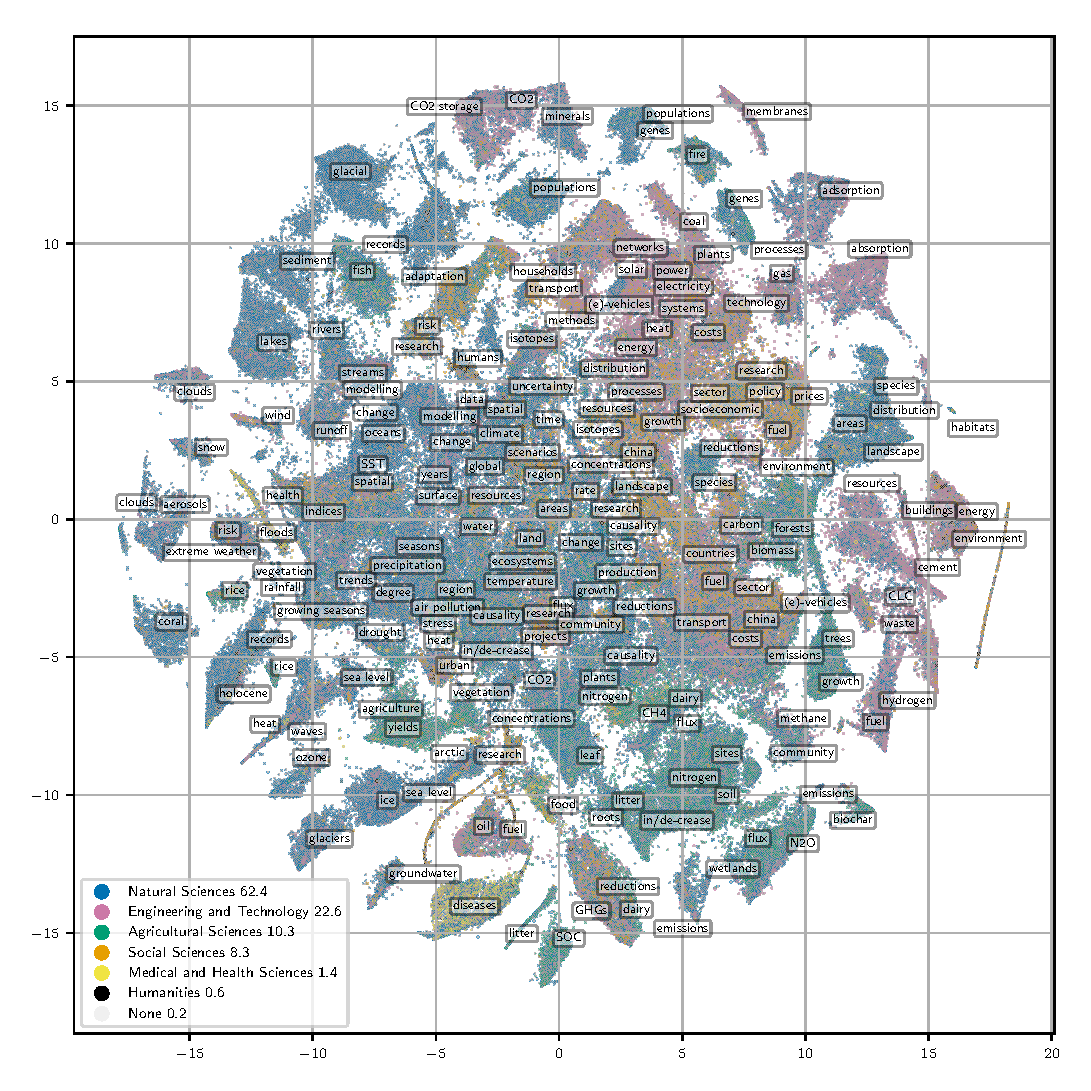
\includegraphics[width=180mm]{plots_pub/all_topic_words_oecds.pdf}
		\caption{A map of the literature on climate change. Document positions are obtained by reducing the topic scores to two dimensions via t-SNE Documents are coloured by web of science discipline category. Topic labels are placed in the center of each of the large clusters of documents associated with each topic. }
		\label{oecd_topic_map}
	\end{center}
\end{figure}

\subsection*{Disciplinary bias in IPCC citations?}

It was argued after the fifth assessment report that the IPCC needed to do more to incorporate knowledge from the social sciences \cite{Victor2015}. Further, a scientometric study from 2011 claimed that the IPCC gave a greater \textit{emphasis} to natural sciences and, within the social sciences, to economics \cite{Bjurström2011}. This claim has been interpreted as a disciplinary bias by the IPCC \cite{Hulme2010, Corbera2016}, but the study operationalised disciplinary emphasis as simply the share of citations from each field, and was based on analysis of the Third Assessment report, published in 2001. The share of citations in each discipline does not take into account the distribution of climate change research across disciplines in the wider literature. Here we look at \textit{representativeness}, that is, the share of IPCC citations in each field divided by the share of all climate related documents in that field, and carry out this analysis across assessment periods.

\begin{figure}[htp]
	\begin{center}
		\includegraphics[width=180mm]{plots_pub/big_panel_representation.pdf}
		\caption{Representation in IPCC reports: \textbf{a)} by discipline, \textbf{b)} by social science proportion of WG 3 topics, \textbf{c)} and novelty of all topics, where topics in the highest and lowest 10\% of either axis are labelled. Topics are coloured according to the working group from which they receive the most citations. Representation is the share of the subset of documents being cited by the IPCC divided by the share of the subset in the whole literature. The log is taken so that 0 is equal to perfectly proportional representation, and -1 and 1 are equally under and over represented.}
		\label{oecd_rep}
	\end{center}
\end{figure}


Looked at this way (Figure 2.a), we see that the social sciences were indeed under-represented in the third assessment report, but by the fifth assessment report were over-represented. The disciplines under-represented in IPCC reports (with respect to the distribution of studies in the wider literature) are in fact Agricultural Sciences, Engineering \& Technology and Humanities (although the humanities make up a very small proportion of the literature). In each field, the under-representation has been present across assessment reports.


A similar story is visible within the social sciences (see figure \ref{subfield}f). 
Economics was previously over-represented among social sciences, while other subfields were under-represented.
In AR5, though, the share of economics citations in the IPCC was close to that in the wider literature, while social \& economic geography (4.3\% of the literature), political science (1.0\%), and sociology (0.8\%) were better represented than in AR3 and above or close to a proportional representation. 

With more up to date data and a more comprehensive method, both results contradict previous evidence on disciplinary representation in the IPCC. This new evidence is a compelling reason to rethink our view of the relationship between disciplinary knowledge and the IPCC. %, and to further investigate the content of the documents that are more less proportionately represented in the IPCC.


\begin{figure}
	\begin{center}
		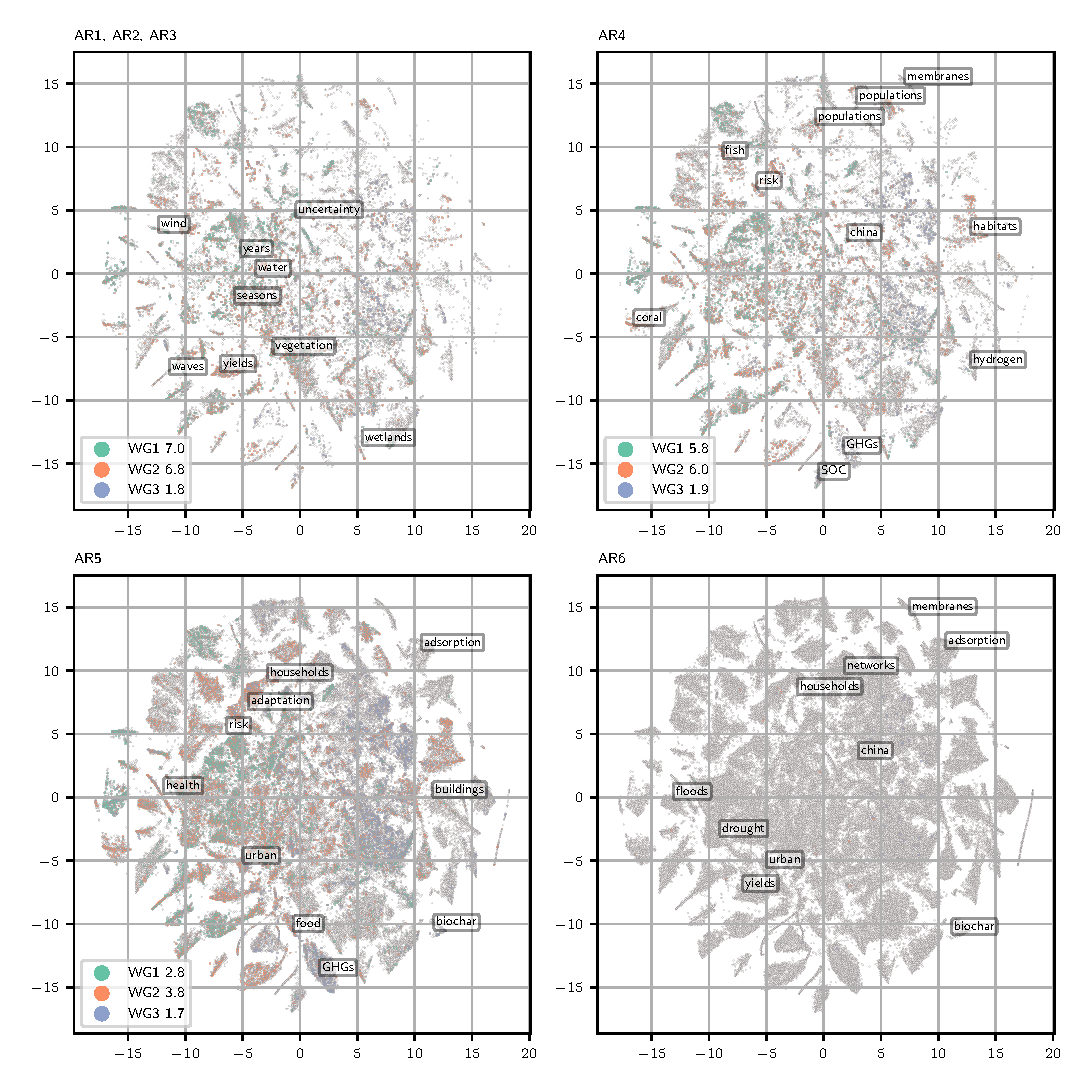
\includegraphics[width=180mm]{plots_pub/topic_evolution_4.pdf}
		\caption{Evolution of the landscape of climate change literature}
		\label{evolution-map}
	\end{center}
\end{figure}

\subsection*{Supply and demand for solutions-oriented knowledge}

Beyond the disciplinary categories analysed so far, the topographical map helps us to dig down further into the themes that are more or less proportionately represented. Figures \ref{oecd_rep}b and \ref{oecd_rep}c plot the representation of the topics. Figure \ref{oecd_rep}c shows that topics more commonly cited by IPCC working group I are older and largely better represented in IPCC reports. It makes intuitive sense that these topics, for example on ozone, oceans, clouds, aerosols and sea levels, are older, predominantly cited by WG I, and well cited by IPCC reports, as these are some of the core topics of the physical science of climate change.

The topics in the lower right of the graph are the most pertinent to the question of whether the IPCC is well representing knowledge on climate change. These topics are newer and until now have been under-represented in IPCC reports. They are the topics that could be seen as potential gaps in the IPCC's coverage of the science. These topics are primarily in working group III, on the mitigation of climate change, with the exception of adsorption, CLC and hydrogen which are primarily of relevance to WG III but are miscategorised due to the low number of citations of relevant documents \footnote{For example, the word ``capacity" is relevant to the adsorption topic, so documents talking about adaptive capacity receive a low relevance score for that topic. Because only very few documents highly relevant to the adsorption topic (in that they talk about adsorption or adsorptive capacity) are cited by the IPCC, and many of the weakly relevant documents are cited by the IPCC, the sum of the topic scores of the weakly relevant WG II documents outweighs the sum of the topic scores of the strongly relevant WG III documents}. and citations of tangentially relevant documents by other working groups

Although it is not surprising that these newer topics are less well represented than the older topics that make up the core of the physical science research on climate change, the difference between these new topics and other new topics that are better represented is intriguing. This difference is visible in figure \ref{evolution-map}, where the fastest growing topics in each period are labelled, and the documents are coloured according to the working group, if any, which cites them. In AR5, the clusters of documents around the \textbf{adsorption}, \textbf{buildings}, and \textbf{biochar} topics contain few IPCC citations, whereas the clusters around \textbf{food}, \textbf{health}, \textbf{adaptation}, and \textbf{GHGs} contain more. This is also evident in figure \ref{oecd_rep}c, where these topics display corresponding representation values. The IPCC, then, has been better at integrating new knowledge from these topics, and in general better at integrating new knowledge from WG II  than WG III topics.

Within WG III topics, those that are well represented contain a greater proportion of social science research (figure \ref{oecd_rep}b). Topics on countries, policy, and prices are close to a proportional representation and are made up of around 30\% social science research. Waste, biochar, cement and coal, are more than 3 times more prevalent in the wider literature than in the literature cited by the IPCC, and are made up of around 5\% social science research. This pattern is not visible in other working groups (see Figure \ref{socsci-wgs}), and complicates the perception of the under-representation of the social sciences.


Recalling policymakers' demands for more solution-oriented assessments \cite{Kowarsch2017}, we could also interpret the topics that are newer and under-represented as ``solutions-relevant''. Many deal with negative emissions, or with mitigation (or to a lesser extent adaptation) options in the transport, buildings and power sectors. All are arguably related to climate solutions. However, while policymakers' demands for solutions-oriented knowledge were rather about policy options, these under-represented new topics deal with more technical solutions.

\subsection*{The IPCC as an informed decision-maker on topical representation}

Deciding on the optimal proportion of each topic's literature to be cited by the IPCC is not a trivial task. A perfectly proportional representation of each topic is almost certainly not optimal, and as such, decisions about which topics to over-, or under- represent are best made by experts, not by a computer. Indeed, the IPCC itself is the best-placed institution to make these decisions. But in the age of ``Big Literature'' \cite{Nunez-Mir2016}, these decision should at best be underpinned by systematic knowledge of the landscape of the literature, and made in discussion with the wider research community, funders, policymakers and other stakeholders.

The analysis in this study provide a useful input to this discussion. It could be argued that the under-represented technical literature on specific technological or sectoral solutions is not relevant to policymakers, and that working group III should give more weight to evidence about general policy instruments such as carbon taxes. Conversely, one could argue that establishing a technical understanding of specific climate solutions is as important a task as establishing a technical understanding of the physical science of climate change. The desire for more social science research in IPCC reports may imply, given the evidence here, that more social science research on climate change needs to be produced and funded, rather than that the IPCC should cite more of what already exists. Or, one could argue that, in light of the evidence that there is little social science research on solutions-relevant, under-represented topics, that the social sciences could do more to address more technical or specific solutions topics such as negative emissions, green concrete, or waste and recycling.

An understanding of the topography of the literature helps bring these arguments to the foreground, and allows them to be made in an informed way. Machine reading the literature in this way is not without its limitations though, and indeed many are apparent in this analysis. The corpus of potentially relevant literature is of course much wider than what is included in this study. The analysis excludes studies about climate change that do not match our query, studies relevant to tackling climate change that do not mention it specifically, studies written in languages other than English (unless the abstract has been translated), studies not indexed in the Web of Science, and reports published outside peer reviewed journals, not to mention Indigenous knowledge \cite{Ford2016b}. Despite this, unless the social science literature in the above categories is systematically less often cited by the IPCC than the social science literature that was analysed in this study, or the solutions-relevant literature in the above categories is systematically more cited by the IPCC, then the two main conclusions of this study hold. 

Ultimately, computers can only \textit{assist} humans in understanding a climate change literature which is produced by human individuals and institutions.  As in other areas of machine learning \cite{Barocas2016}, computational assessments of the literature run the risk of reproducing biases or gaps in the training data. However, just as with other applications of machine learning, machine-reading the science of climate change can provide information that helps us to understand gaps in what we have knowledge about, and potential biases, or options for emphasis, in how we represent that knowledge in the IPCC. %Machine learning approaches to understanding scientific literature are already latently present in our engagement with  when we use academic search engines or are recommended articles 

\end{linenumbers}

\appendix

%\listoffigures
\linespread{1}
%\bibliography{Mendeley}
\begin{thebibliography}{10}
	
	\bibitem{Bjurström2011}
	Andreas Bjurstr{\"{o}}m and Merritt Polk.
	\newblock {Physical and economic bias in climate change research: A
		scientometric study of IPCC Third Assessment Report}.
	\newblock {\em Climatic Change}, 108(1):1--22, 2011.
	
	\bibitem{Grieneisen2011}
	Michael Grieneisen and Minghua Zhang.
	\newblock {The Current Status of Climate Change Research}.
	\newblock {\em Nature Climate Change}, 1:72--73, 2011.
	
	\bibitem{Haunschild2016}
	Robin Haunschild, Lutz Bornmann, and Werner Marx.
	\newblock {Climate Change Research in View of Bibliometrics}.
	\newblock {\em PLoS ONE}, 11(7):1--19, 2016.
	
	\bibitem{Minx2017l}
	Jan~C. Minx, Max Callaghan, William~F. Lamb, Jennifer Garard, and Ottmar
	Edenhofer.
	\newblock {Learning about climate change solutions in the IPCC and beyond}.
	\newblock {\em Environmental Science {\&} Policy}, 2017.
	
	\bibitem{Kowarsch2017}
	Martin Kowarsch, Jason Jabbour, Christian Flachsland, Marcel T.~J. Kok, Robert
	Watson, Peter~M. Haas, Jan~C. Minx, Joseph Alcamo, Jennifer Garard, Pauline
	Riousset, L{\'{a}}szl{\'{o}} Pint{\'{e}}r, Cameron Langford, Yulia Yamineva,
	Christoph von Stechow, Jessica O'Reilly, and Ottmar Edenhofer.
	\newblock {A road map for global environmental assessments}.
	\newblock {\em Nature Climate Change}, 7(6):379--382, 2017.
	
	\bibitem{Victor2015}
	{David G. Victor}.
	\newblock {Embed the social sciences in climate policy - David Victor}.
	\newblock {\em Nature}, 520:7--9, 2015.
	
	\bibitem{Barnes2013}
	Jessica Barnes, Michael Dove, Myanna Lahsen, Andrew Mathews, Pamela McElwee,
	Roderick McIntosh, Frances Moore, Jessica O'Reilly, Ben Orlove, Rajindra
	Puri, Harvey Weiss, and Karina Yager.
	\newblock {Contribution of anthropology to the study of climate change}.
	\newblock {\em Nature Climate Change}, 3(6):541--544, 2013.
	
	\bibitem{Hulme2010}
	Mike Hulme and Martin Mahony.
	\newblock {Climate change: What do we know about the IPCC?}
	\newblock {\em Progress in Physical Geography}, 34(5):705--718, 2010.
	
	\bibitem{Blei2012}
	David Blei, Lawrence Carin, and David Dunson.
	\newblock {Probabilistic topic models}.
	\newblock {\em Communications of the ACM}, 55(4):77--84, 2012.
	
	\bibitem{vandermaaten2008}
	Laurens van~der Maaten and Geoffrey Hinton.
	\newblock {Visualizing Data using t-SNE}.
	\newblock {\em Journal of Machine Learning Research}, 9:2579--2605, 2008.
	
	\bibitem{Edenhofer2015}
	Ottmar Edenhofer and Martin Kowarsch.
	\newblock {Cartography of pathways: A new model for environmental policy
		assessments}.
	\newblock {\em Environmental Science and Policy}, 51:56--64, 2015.
	
	\bibitem{McKinnon2015}
	Madeleine~C McKinnon, Samantha~H Cheng, Ruth Garside, Yuta~J Masuda, and
	Daniel~C Miller.
	\newblock {Sustainability: Map the evidence}.
	\newblock {\em Nature}, 528(7581):185--187, 2015.
	
	\bibitem{James2016}
	Katy~L. James, Nicola~P. Randall, and Neal~R. Haddaway.
	\newblock {A methodology for systematic mapping in environmental sciences}.
	\newblock {\em Environmental Evidence}, 5(1):1--13, 2016.
	
	\bibitem{Corbera2016}
	Esteve Corbera, Laura Calvet-Mir, Hannah Hughes, and Matthew Paterson.
	\newblock {Patterns of authorship in the IPCC Working Group III report}.
	\newblock {\em Nature Climate Change}, 6(1):94--99, 2016.
	
	\bibitem{Nunez-Mir2016}
	Gabriela~C. Nunez-Mir, Basil~V. Iannone, Bryan~C. Pijanowski, Ningning Kong,
	Songlin Fei, and Richard Fitzjohn.
	\newblock {Automated content analysis: addressing the big literature challenge
		in ecology and evolution}.
	\newblock {\em Methods in Ecology and Evolution}, 7(11):1262--1272, 2016.
	
	\bibitem{Ford2016b}
	James~D. Ford, Laura Cameron, Jennifer Rubis, Michelle Maillet, Douglas
	Nakashima, Ashlee~Cunsolo Willox, and Tristan Pearce.
	\newblock {Including indigenous knowledge and experience in IPCC assessment
		reports}.
	\newblock {\em Nature Climate Change}, 6(4):349--353, 2016.
	
	\bibitem{Barocas2016}
	Solon Barocas and Andrew~D Selbst.
	\newblock {Big Data's Disparate Impact}.
	\newblock {\em California Law Review}, 104:671--732, 2016.
	
\end{thebibliography}
\bibliographystyle{unsrt}

%\documentclass{article}
\usepackage[a4paper, total={6in, 8in}]{geometry}
\usepackage{graphicx}
\usepackage{url}
\usepackage{natbib}
\usepackage{todonotes}
\usepackage{booktabs}
\usepackage{lineno}
\usepackage{color}
%\usepackage{auto-pst-pdf}
\usepackage[colaction]{multicol}
\usepackage{caption}
\usepackage{svg}
\usepackage{authblk}
\usepackage{standalone}
\usepackage[section]{placeins}

\makeatletter
\renewcommand{\maketitle}{\bgroup\setlength{\parindent}{0pt}
	\begin{flushleft}
		
		{\huge\textbf{\@title}}
		
		\bigskip
		
		{\large\textbf{\@author}}
		
		\bigskip
		
		{\large{Draft current \@date}}
		
	\end{flushleft}\egroup
}
\makeatother


\begin{document}
	% Title
	\title{A Topic Model of Climate Change Literature}
	\title{Words, words, words: Mapping the Matter of Climate Change Literature}
	\title{A Topography of Climate Change Research - Methods}
	\author[1,2]{Max Callaghan}
	
	\affil[1]{Mercator Research Institute on Global Commons and Climate Change, Torgauer Straße, 10829 Berlin, Germany}
	\affil[2]{School of Earth and Environment, University of Leeds, Leeds LS2 9JT, United Kingdom}
	\maketitle
	\begin{linenumbers}
	
	\setcounter{figure}{0}
	\renewcommand\thefigure{SI.\arabic{figure}}  
		
	\subsection*{Data}
	
	This study reproduces the query developed by \citep{Grieneisen2011}, which is carried out on the Web of Science core collection. Though not exhaustive, the Web of Science gives a good coverage of the literature in major peer-reviewed journals.	Each document is assigned to an assessment period according to the timeline shown in table 1.
	
	We use the references scraped from IPCC assessment reports from \citep{Minx2017l}, and attempt to match these with the results from the web of science. Table \todo{}[x] shows the percentage of IPCC citations matched in each working group for each assessment report.
		
	\subsection*{Pre-processing}
	
	Data quality in earlier Web of Science results is poorer, and some documents have missing abstracts. In the quantification of the size of the literature and its vocabulary in table [], titles are substituted for abstracts where they are not available.  The words of the documents are lemmatized/stemmed, replacing different forms of the same word (i.e. word/words) with a single instance. Commonly occuring words, or ``stopwords'' are removed, as are all words shorter than 3 characters, and all words containing only punctuation or numbers.
	
	The documents are transformed into a document-term matrix, where each row represents a document, and each column represents a unique word.  Each cell contains the number of that column's terms in that document. Only terms which occur more than once are considered.
	
	For the calculation of the topic model, documents with missing abstracts are ignored, and the document term matrix is transformed into a document
	frequency-inverse document frequency (tf-idf) matrix, where scores are scaled according to the frequency of their occurence in the corpus. This gives more weight to terms which appear in few documents, and less weight to those which appear in many.
	
	\begin{equation}
	tf(t,d) = f_{t,d} \mathrm{,}\quad idf(t,D) = \log\frac{N}{|\{d \in D:t \in d\}|}
	\end{equation} 
	
	\subsection*{Topic Model}
	
	We use non-negative Matrix Factorisation (NMF) \cite{Lee1999}, an approach to topic modelling which factorises the term-frequency-inverse document frequency matrix \( V \) into the matrices \(W\), the topic-term matrix, and \( H \) the document-topic matrix, whose product approximates \(V\):
	
	\begin{equation}
		V_{i\mu} \approx (WH)_{i\mu} = \sum_{a=1}^{r}W_{ia}H_{a\mu}
	\end{equation}
	
	As demonstrated in Figure \ref{doc-topic}, each topic is represented as a set of word scores, and each document a set of topic scores. The combination of the two give the word scores in the document. For clarity in the figure, these are shown as simple counts, but in the model these are scaled according to each term's frequency within the corpus as explained above.
	
	Topics are calculated using the scikitlearn library \cite{Pedregosa2011}, and are saved in a database and topic visualisation system based on \cite{Chaney2012} \footnote{The system adds new functionality to \cite{Chaney2012} and combines it with a system for managing sets of documents and queries. The code and additional information is published online at \url{https://github.com/mcallaghan/tmv}}. 	
	
	\subsubsection*{Model selection}
	
	Topic models are calculated for 70, 80, 90, 100, 110, 120, 130 and 140 topics. The relative usefulness of each model was assessed subjectively by the authors, based on inspection of the online visualisation tool, and the spreadsheet \textbf{topic\_comparison.xlsx} accompanying the supporting information. The spreadsheet shows each set of topics in adjacent columns. Topics from each model are placed next to the topics with the largest number of each topic's 10 highest scoring words in common. This helps authors to find an appropriate level of granularity for the analysis. 
			
	\subsubsection*{Topic Representation and Newness}
	
	To calculate topic representation in IPCC reports we divide each topic's share in the subsample of documents cited by IPCC reports by its share in the whole corpus. 
	
	We calculate a topic's total score as the sum of document-topic scores. A topic's window score is the sum of document-topic scores considering only documents in the given time window. To represent a topic's newness, we multiply each assessment period number by the share of it's total score occurring in that window, and take the mean of these scores. A topic in which 100\% of documents which make it up occurred in assessment period 1 (6) would thereby receive a score of 1 (6), while a topic evenly distributed across all assessment periods would receive a score of 3.5.
	
	
	\subsubsection*{Disciplinary Entropy}
	
	Disciplinary Entropy inverts the measurement of a conference's topical diversity suggested in \cite{Hall2008}, by measuring a topic \(z\)'s entropy \(H\), where 
	
	\begin{equation}
		H(f|z) = -\sum_{i=1}^K \hat{p}(f|z) \log \hat{p}(f|z) 
	\end{equation}
	
	based on the empirical distribution of a field \(f\) in the documents \(d\) in each topic:
	
	\begin{equation}
		\hat{p}(f|z) = \sum_{d:z_d=z} \hat{p} (f|d) \hat{p} (d|z)
	\end{equation}

	\begin{figure}
		\begin{center}
			\includegraphics[width=1\linewidth]{plots_pub/topic_oecd_entropy.pdf}
			\caption{SI Disciplinary Entropy}
			\label{dis-entropy}
		\end{center}
	\end{figure}	
	
	
	
	\begin{figure}
		\begin{center}
			\includegraphics[width=1\linewidth]{plots_pub/single_doc_3_536594_1861.pdf}
			\caption{SI Topic make up of a single document}
			\label{doc-topic}
		\end{center}
	\end{figure}

	\begin{figure}
	\begin{center}
		\includegraphics[width=1\linewidth]{plots_pub/ipcc_rep_wcs_simplified.pdf}
		\caption{SI Representation by subfield}
		\label{subfield}
	\end{center}
\end{figure}

\begin{figure}
	\begin{center}
		\includegraphics[width=1\linewidth]{plots_pub/wgs_socsci.pdf}
		\caption{SI Social science \& representation in topics across working groups}
		\label{socsci-wgs}
	\end{center}
\end{figure}

\subsection*{Glossary}


\noindent\textbf{ncep:} National Centers for Environmental Protection

\noindent\textbf{fco:} Fugacity of Carbon Dioxide

\noindent\textbf{pfc:} Perflourocompound

\noindent\textbf{otcs:} Open Top Chambers

\noindent\textbf{dtr:} Diurnal Temperature Range

\noindent\textbf{sres:} Special Report on Emissions Scenarios (200)

\noindent\textbf{petm:} Paleocene Eocene Thermal Maximum

\noindent\textbf{amf:}  Arbuscular Mycorrhizal Fungal

\noindent\textbf{sf5cf3:} trifluoromethyl sulfur pentafluoride (A Potent Greenhouse Gas Identified in the Atmosphere, 2000)

\noindent\textbf{clc:} Chemical Looping Combustion

\noindent\textbf{cwd:} Coarse woody debris

\noindent\textbf{etm:} Enhanced Thematic Mapper (NASA satellite sensor)

\noindent\textbf{cmip5:} Coupled Model Intercomparison Project 5 (Starting 2008)

\noindent\textbf{cmip3:} Coupled Model Intercomparison Project phase 3 (first published 2007 \cite{Meehl2007})

\noindent\textbf{mofs:} metal-organic frameworks (for CO2 storage)

\noindent\textbf{sdm:} statistical-dynamical model

\noindent\textbf{mmms:} Mixed Matrix Membranes (for CO2 capture)

\noindent\textbf{cop21:} 21st Conference of Parties (Paris 2015) 

\noindent\textbf{c3n4:} Carbon nitride (a synthetic nanomaterial used for hydrogen production)

\noindent\textbf{sdg:} Sustainable Development Goals

\noindent\textbf{indc:} Intended Nationally Determined Contributions

		
	\end{linenumbers}

\linespread{1}
%\bibliography{Mendeley}

\begin{thebibliography}{1}
	
	\bibitem{Grieneisen2011}
	Michael Grieneisen and Minghua Zhang.
	\newblock {The Current Status of Climate Change Research}.
	\newblock {\em Nature Climate Change}, 1:72--73, 2011.
	
	\bibitem{Minx2017l}
	Jan~C. Minx, Max Callaghan, William~F. Lamb, Jennifer Garard, and Ottmar
	Edenhofer.
	\newblock {Learning about climate change solutions in the IPCC and beyond}.
	\newblock {\em Environmental Science {\&} Policy}, 2017.
	
	\bibitem{Lee1999}
	D~D Lee and H~S Seung.
	\newblock {Learning the parts of objects by non-negative matrix factorization.}
	\newblock {\em Nature}, 401(6755):788--91, 1999.
	
	\bibitem{Pedregosa2011}
	Fabian Pedregosa, Ga{\"{e}}l Varoquaux, Alexandre Gramfort, Vincent Michel,
	Bertrand Thirion, Olivier Grisel, Mathieu Blondel, Peter Prettenhofer, Ron
	Weiss, Vincent Dubourg, Jake Vanderplas, Alexandre Passos, David Cournapeau,
	Matthieu Brucher, Mattheiu Perrot, and {\'{E}}douard Duchesnay.
	\newblock {Scikit-learn: Machine Learning in Python Fabian}.
	\newblock {\em Journal of Machine Learning Research}, 12:2825--2830, 2011.
	
	\bibitem{Chaney2012}
	Allison J~B Chaney and David~M. Blei.
	\newblock {Visualizing Topic Models}.
	\newblock {\em Icwsm}, pages 419--422, 2012.
	
	\bibitem{Hall2008}
	David Hall, Daniel Jurafsky, and Christopher~D. Manning.
	\newblock {Studying the history of ideas using topic models}.
	\newblock {\em Proceedings of the Conference on Empirical Methods in Natural
		Language Processing - EMNLP '08}, pages 363--371, 2008.
	
	\bibitem{Meehl2007}
	Gerald~A. Meehl, Curt Covey, Thomas Delworth, Mojib Latif, Bryant McAvaney,
	John~F.B. Mitchell, Ronald~J. Stouffer, and Karl~E. Taylor.
	\newblock {The WCRP CMIP3 multimodel dataset: A new era in climatic change
		research}.
	\newblock {\em Bulletin of the American Meteorological Society},
	88(9):1383--1394, 2007.
	
\end{thebibliography}


\bibliographystyle{unsrt}

\end{document}

\end{document}